\documentclass[11pt]{article}

\usepackage[margin=1in]{geometry}
\usepackage{amsmath, amssymb}
\usepackage[utf8]{inputenc}
\usepackage[T1]{fontenc}
\usepackage{lmodern}
\usepackage{microtype}
\usepackage{graphicx}
\usepackage{booktabs}
\usepackage{array}
\usepackage{tabularx}
\usepackage{textcomp}
\usepackage{float}
\usepackage{xcolor}
\usepackage{fancyhdr}
\usepackage[font=small,labelfont=bf,skip=5pt]{caption}
\usepackage{listings}
\lstdefinestyle{pycode}{
  language=Python, basicstyle=\ttfamily\scriptsize,
  keywordstyle=\color{psink}\bfseries, commentstyle=\color{psaccent}\itshape,
  stringstyle=\color{psink}, numbers=left, numberstyle=\tiny\color{psrule},
  numbersep=7pt, breaklines=true, breakatwhitespace=true, showstringspaces=false,
  frame=none, xleftmargin=20pt, aboveskip=6pt, belowskip=6pt, columns=fullflexible,
  keepspaces=true, upquote=true,
}
\lstset{style=pycode}

\definecolor{psink}{RGB}{23,54,93}
\definecolor{psaccent}{RGB}{192,80,77}
\definecolor{psrule}{RGB}{200,209,222}

\usepackage[colorlinks=true,allcolors=psink]{hyperref}

\graphicspath{{./}}
\newcommand{\ex}{\mathrm{e}}   % used in questions (d)-(e)
\emergencystretch=3em

\setlength{\textfloatsep}{10pt plus 2pt minus 2pt}
\setlength{\intextsep}{10pt plus 2pt minus 2pt}
\setlength{\abovecaptionskip}{4pt}
\setlength{\belowcaptionskip}{0pt}

\makeatletter
\renewcommand\section{\@startsection{section}{1}{0pt}%
  {-2.6ex \@plus -1ex \@minus -.2ex}{1.3ex \@plus .2ex}%
  {\normalfont\scshape\large\color{psink}}}   % lmr has no bold small caps
\renewcommand\subsection{\@startsection{subsection}{2}{0pt}%
  {-2.2ex \@plus -1ex \@minus -.2ex}{1.0ex \@plus .2ex}%
  {\normalfont\bfseries\normalsize\color{psink}}}
\renewcommand\subsubsection{\@startsection{subsubsection}{3}{0pt}%
  {-1.9ex \@plus -.8ex \@minus -.2ex}{0.8ex \@plus .2ex}%
  {\normalfont\bfseries\itshape\normalsize\color{psink}}}
\renewcommand\subparagraph{\@startsection{subparagraph}{5}{0pt}%
  {-1.6ex \@plus -.6ex \@minus -.2ex}{0.5ex \@plus .1ex}%
  {\normalfont\itshape\normalsize\color{psink}}}
\renewcommand\paragraph{\@startsection{paragraph}{4}{0pt}%
  {1.7ex \@plus 1ex \@minus .2ex}{-0.9em}%
  {\normalfont\bfseries\normalsize\color{psink}}}
\makeatother

\newenvironment{tight}
  {\begin{itemize}\setlength{\itemsep}{3pt}\setlength{\parskip}{0pt}%
   \setlength{\topsep}{3pt}\setlength{\leftmargini}{1.4em}}
  {\end{itemize}}

\setcounter{secnumdepth}{0}   % headings carry the assignment's own labels
\setlength{\headheight}{22pt}
\pagestyle{fancy}
\fancyhf{}
\fancyhead[L]{\footnotesize\scshape\color{psink} MGT 595 \textemdash\ Problem Set 8}
\fancyhead[R]{\footnotesize\color{psink}\thepage}
\renewcommand{\headrulewidth}{0.4pt}
\renewcommand{\headrule}{\hbox to\headwidth{%
  \color{psrule}\leaders\hrule height \headrulewidth\hfill}}

\begin{document}

\thispagestyle{empty}
\begin{flushleft}
{\bfseries\LARGE\color{psink} Quantitative Investing}\\[3pt]
{\scshape\Large\color{psink} Problem Set 8}\\[10pt]
{\color{psrule}\rule{\textwidth}{1.2pt}}\\[5pt]
{\small Ashley Wen\,(xw564)\quad\textbar\quad Emily Wu\,(esw63)%
\quad\textbar\quad Grace Gu\,(xg325)\hfill \today}
\end{flushleft}

\vspace{1.4em}

{\color{psink}\textbf{Contents.}} Questions (a)--(c) document the January and December
seasonals in the 75 size and past-return portfolios and discuss what they mean for market
efficiency. Questions (d)--(e) run Fama--MacBeth regressions on past returns and build a
pre-registered trading strategy, tuned on 1953--2001 and tested on 2001--2026. Questions
(f)--(g) put confidence intervals around that strategy's Sharpe ratio and compare it with
5,000 random strategies, including the AI integration exercises on data mining.

\vspace{0.8em}

% Problem Set 8 -- Part 1: questions (a), (b), (c). Numbers from ps8_partA.py.

\section{Questions (a)--(c): Seasonality in Returns}

All regressions use the 75 portfolios sorted on size and past 1-month, 2--12-month and
13--60-month returns. The left-hand side is the portfolio return in excess of the T-bill, in
\% per month. The sample is 1931:02--2026:06 ($T=1{,}145$), the months in which all three
sorts exist. Four portfolios have a few months coded $-99.99$, which we drop, so their $T$ is
slightly smaller (at least 1{,}127).

\subsection*{Question (a): the January seasonal}

We run $r^e_{i,t} = c_i + J_i\,\mathrm{Jan}_t + \varepsilon_{i,t}$ for each portfolio. The
intercept $c_i$ is the mean excess return from February to December, and $J_i$ is the extra
January return. Table~\ref{tab:jan} reports $J_i$ for all 75 portfolios.

\begin{table}[H]
\centering\small
\caption{January premium $J_i$ (\% per month) from $r^e_{i,t}=c_i+J_i\,\mathrm{Jan}_t+\varepsilon_{i,t}$, OLS $t$-statistics in parentheses. Rows are size quintiles, columns are past-return quintiles (Low = past losers, High = past winners). 1931:02--2026:06.}
\label{tab:jan}
\begin{tabular}{lccccc}
\toprule
Size & Low & 2 & 3 & 4 & High \\
\midrule
\multicolumn{6}{l}{\textit{Panel A: sorted on past 1-month return}} \\
Small & 7.32 (6.5) & 4.74 (4.8) & 4.15 (4.3) & 3.72 (4.1) & 3.49 (3.7) \\
2 & 3.92 (4.0) & 3.05 (3.7) & 2.33 (3.0) & 2.14 (2.6) & 1.32 (1.6) \\
3 & 3.02 (3.4) & 2.35 (3.1) & 1.78 (2.5) & 1.44 (2.1) & 0.39 (0.5) \\
4 & 2.15 (2.6) & 1.69 (2.4) & 1.21 (1.9) & 0.40 (0.6) & $-$0.10 ($-$0.1) \\
Big & 1.16 (1.6) & 0.54 (0.9) & 0.15 (0.3) & $-$0.11 ($-$0.2) & $-$0.52 ($-$0.8) \\
\midrule
\multicolumn{6}{l}{\textit{Panel B: sorted on past 2--12-month return}} \\
Small & 7.45 (6.7) & 5.14 (5.3) & 4.32 (4.8) & 3.56 (3.8) & 3.57 (3.9) \\
2 & 4.07 (3.9) & 3.10 (3.6) & 2.38 (3.1) & 1.68 (2.2) & 1.66 (2.0) \\
3 & 2.95 (3.0) & 2.10 (2.6) & 1.68 (2.3) & 1.15 (1.7) & 0.91 (1.3) \\
4 & 2.23 (2.2) & 1.45 (1.9) & 0.95 (1.4) & 0.39 (0.6) & 0.34 (0.5) \\
Big & 1.69 (1.9) & 0.82 (1.2) & 0.13 (0.2) & $-$0.32 ($-$0.6) & $-$0.55 ($-$0.9) \\
\midrule
\multicolumn{6}{l}{\textit{Panel C: sorted on past 13--60-month return}} \\
Small & 7.42 (6.9) & 4.73 (5.1) & 3.45 (4.0) & 4.24 (4.6) & 3.70 (3.7) \\
2 & 4.56 (4.6) & 2.90 (3.4) & 2.08 (2.7) & 1.71 (2.1) & 1.61 (1.9) \\
3 & 3.82 (4.1) & 2.17 (2.8) & 1.73 (2.4) & 1.23 (1.8) & 0.99 (1.3) \\
4 & 2.67 (3.0) & 1.29 (1.7) & 1.20 (1.7) & 0.77 (1.1) & 0.28 (0.4) \\
Big & 2.06 (3.1) & 0.72 (1.2) & 0.31 (0.5) & $-$0.15 ($-$0.3) & $-$0.34 ($-$0.6) \\
\bottomrule
\end{tabular}
\end{table}

\begin{tight}
  \item \textbf{Is there a strong January seasonal different from other months?} Yes, January
  is by far the strongest month for most of these portfolios. The January premium is positive
  and significant ($t>2$) in 43 of the 75 portfolios, and across all 75 it averages 2.1\% on
  top of a February--December mean of about 0.8\%. In other words, an average portfolio earns
  almost four times its normal monthly return in January.

  \item \textbf{For which portfolios is this largest or smallest?} The effect is largest for
  small past losers and disappears for large past winners. In every panel the January premium
  generally falls as we move from small to big stocks and from losers to winners, so the small--loser
  corner earns more than 7\% extra in January with $t$-statistics near 7. The big--winner
  corner has a small negative premium that is not significant. The pattern looks the same
  whether ``losers'' are defined over 1, 12 or 60 months, so the January effect is a
  small-stock and past-loser effect at every horizon.

  \item \textbf{Why might this be?} The most common explanation is tax-loss selling. Investors
  sell stocks with capital losses in December to cut their tax bill, which pushes down prices
  of past losers, and then buy back in January when the selling pressure ends. Small stocks are
  hit hardest because they are illiquid, held mostly by taxable individuals, and expensive to
  arbitrage. Window dressing adds to this: fund managers dump embarrassing losers before
  year-end reports and buy riskier small stocks again in January. The intercepts also show that
  past 12-month losers earn only 0.1--0.3\% per month from February to December against
  1.0--1.3\% for winners, so momentum is a February--December phenomenon that reverses in
  January. All of
  these stories point to year-end trading pressure, not a change in risk, as the source of the
  January return.
\end{tight}

\subsection*{Question (b): adding December}

We add a December dummy,
$r^e_{i,t} = c_i + J_i\,\mathrm{Jan}_t + D_i\,\mathrm{Dec}_t + \varepsilon_{i,t}$, so $c_i$ is
now the February--November mean. Table~\ref{tab:dec} reports $D_i$ for all 75 portfolios, and
Table~\ref{tab:corners} compares the three means in the four corner portfolios.

\begin{table}[H]
\centering\small
\caption{December premium $D_i$ (\% per month) from $r^e_{i,t}=c_i+J_i\,\mathrm{Jan}_t+D_i\,\mathrm{Dec}_t+\varepsilon_{i,t}$, OLS $t$-statistics in parentheses. Layout as in Table~\ref{tab:jan}.}
\label{tab:dec}
\begin{tabular}{lccccc}
\toprule
Size & Low & 2 & 3 & 4 & High \\
\midrule
\multicolumn{6}{l}{\textit{Panel A: sorted on past 1-month return}} \\
Small & $-$0.12 ($-$0.1) & 0.10 (0.1) & $-$0.06 ($-$0.1) & $-$0.01 (0.0) & 0.29 (0.3) \\
2 & 0.68 (0.7) & 0.76 (0.9) & 0.74 (0.9) & 0.99 (1.2) & 1.11 (1.3) \\
3 & 1.02 (1.1) & 0.69 (0.9) & 1.12 (1.6) & 1.02 (1.5) & 1.03 (1.3) \\
4 & 0.94 (1.1) & 0.80 (1.2) & 1.16 (1.8) & 0.94 (1.4) & 1.17 (1.6) \\
Big & 0.43 (0.6) & 0.52 (0.9) & 0.67 (1.2) & 0.78 (1.4) & 0.60 (0.9) \\
\midrule
\multicolumn{6}{l}{\textit{Panel B: sorted on past 2--12-month return}} \\
Small & $-$0.65 ($-$0.6) & $-$0.32 ($-$0.3) & $-$0.24 ($-$0.3) & 0.30 (0.3) & 1.00 (1.1) \\
2 & 0.16 (0.2) & 0.35 (0.4) & 0.79 (1.0) & 1.39 (1.8) & 1.46 (1.8) \\
3 & 0.62 (0.6) & 0.66 (0.8) & 0.68 (0.9) & 1.27 (1.9) & 1.48 (2.0) \\
4 & 0.34 (0.3) & 0.61 (0.8) & 0.79 (1.2) & 1.13 (1.8) & 1.60 (2.4) \\
Big & $-$0.60 ($-$0.7) & $-$0.01 (0.0) & 0.52 (0.9) & 0.90 (1.6) & 1.19 (2.0) \\
\midrule
\multicolumn{6}{l}{\textit{Panel C: sorted on past 13--60-month return}} \\
Small & $-$0.31 ($-$0.3) & 0.07 (0.1) & 0.22 (0.2) & $-$0.10 ($-$0.1) & 0.07 (0.1) \\
2 & 0.58 (0.6) & 0.91 (1.1) & 0.94 (1.2) & 0.75 (0.9) & 0.51 (0.6) \\
3 & 1.00 (1.1) & 0.92 (1.2) & 1.10 (1.5) & 0.71 (1.0) & 0.74 (1.0) \\
4 & 0.66 (0.7) & 0.80 (1.1) & 0.98 (1.4) & 1.03 (1.5) & 0.87 (1.2) \\
Big & 0.65 (1.0) & 0.68 (1.1) & 0.54 (0.9) & 0.67 (1.1) & 0.39 (0.6) \\
\bottomrule
\end{tabular}
\end{table}

\begin{table}[H]
\centering\small
\caption{Corner portfolios from the January--December regression. $c$ is the February--November mean, $J$ and $D$ are the extra January and December returns (\% per month, $t$ in parentheses), and the last column is the $t$-statistic of $J-D$.}
\label{tab:corners}
\begin{tabular}{llcccc}
\toprule
Sort & Portfolio & Feb--Nov $c$ & January $J$ & December $D$ & $t(J-D)$ \\
\midrule
1-month & Small, low & 1.42 & 7.31 (6.5) & $-$0.12 ($-$0.1) & 4.9 \\
 & Small, high & $-$0.23 & 3.51 (3.7) & 0.29 (0.3) & 2.5 \\
 & Big, low & 0.70 & 1.20 (1.6) & 0.43 (0.6) & 0.8 \\
 & Big, high & 0.47 & $-$0.46 ($-$0.7) & 0.60 (0.9) & $-$1.2 \\
\addlinespace
2--12-month & Small, low & 0.12 & 7.39 (6.6) & $-$0.65 ($-$0.6) & 5.3 \\
 & Small, high & 1.15 & 3.66 (4.0) & 1.00 (1.1) & 2.2 \\
 & Big, low & 0.36 & 1.64 (1.8) & $-$0.60 ($-$0.7) & 1.8 \\
 & Big, high & 0.89 & $-$0.44 ($-$0.7) & 1.19 (2.0) & $-$2.0 \\
\addlinespace
13--60-month & Small, low & 0.85 & 7.39 (6.8) & $-$0.31 ($-$0.3) & 5.3 \\
 & Small, high & 0.50 & 3.70 (3.7) & 0.07 (0.1) & 2.7 \\
 & Big, low & 0.57 & 2.12 (3.2) & 0.65 (1.0) & 1.6 \\
 & Big, high & 0.63 & $-$0.31 ($-$0.5) & 0.39 (0.6) & $-$0.8 \\
\bottomrule
\end{tabular}
\end{table}

\begin{tight}
  \item \textbf{Is there a strong December and January seasonal, and are they different from
  each other?} Yes for January, but December is only a modest seasonal, and the two are
  clearly different for small stocks. Adding the December dummy barely changes the January
  premia. December premia are mostly positive, averaging 0.6\% across the 75 portfolios, but
  only 2 of 75 have $t>2$ with OLS standard errors. December is a calmer month than the rest of
  the year, so with White standard errors 12 portfolios reach $t>2$, 8 of them 12-month winners.
  December is therefore a real but modest seasonal, about 1--1.6\% in a few portfolios. January exceeds December significantly in 21 portfolios, all but one of them in
  the two smallest size quintiles, while for big stocks the two months cannot be told apart.

  \item \textbf{For which portfolios are these seasonalities largest or smallest?} The two
  seasonals run in opposite directions across portfolios. The January effect is largest for
  small losers, while December is weakest there: small stocks earn nothing significant extra in December,
  and small 12-month losers are even slightly negative. December is largest for mid-to-large
  12-month winners, where it is about 1--1.6\% and significant with White standard errors, and these are
  exactly the portfolios with no significant January effect. So small losers do badly into year-end and then rebound,
  while large winners do well into year-end and, if anything, give a little back in January.

  \item \textbf{Can you conjecture why these differences exist?} The mirror-image pattern is
  what year-end selling pressure would produce. In December, tax-loss sellers and window
  dressers sell losers and hold or buy winners, so losers lag and winners gain. In January the
  pressure lifts, and the losers bounce back while winners are sold to realize gains in the new
  tax year. The effect concentrates in small stocks because their prices move most for a given
  amount of selling. The December premium in mid and large stocks may also reflect the
  pre-holiday effect and year-end inflows into the broad market, which would explain why mid
  and large stocks earn a little extra in December across most past-return groups.
\end{tight}

\subsection*{Question (c): market efficiency}

\begin{tight}
  \item \textbf{Are these findings evidence for or against market efficiency?} At face value
  they are evidence against it, but weaker evidence than the $t$-statistics suggest. A return
  pattern tied to the calendar is known in advance, so in an efficient market investors should
  buy small losers in late December and trade the January premium away. Its strength over 95 years, at
  $t$-statistics near 7, is hard to explain with risk. Still, several caveats
  below mean the findings do not cleanly reject efficiency.

  \item \textbf{How would you try to reconcile them with the efficient markets hypothesis?}
  There are three ways. First, statistics: we looked at 75 portfolios and could have tested
  any of 12 months, so some large $t$-statistics are expected by chance. The effect has also
  weakened sharply since it was published in the late 1970s and early 1980s: the January
  premium is significant in 46 of 75 portfolios before 1983 but in only 6 after, which is what
  we would expect if investors learned about it and traded it away. Second, transaction costs: small losers
  have wide bid--ask spreads and low prices, so the premium may not survive realistic trading
  costs and short-sale limits. Third, the model: we assumed expected returns are constant across
  months, and EMH only says prices reflect information given the right model of risk. If small
  stocks carry more risk in January, or if taxes make the after-tax return equal across months,
  then a higher pre-tax January return is just compensation. This is the joint-hypothesis
  problem: we are always testing efficiency and the risk model together.

  \item \textbf{How are the findings perhaps a violation of efficient markets?} The risk story
  is hard to defend, because nothing about a firm's risk changes on January 1. The tax story
  only explains why some investors sell, not why arbitrageurs without tax motives fail to buy.
  The effect is also very large relative to normal returns and has been documented in many
  countries, including ones with different tax years (Gultekin and Gultekin, 1983), which makes pure data mining less
  likely. If the premium survives after costs, it is a violation at least of the weak form,
  since the signal uses only past prices and the calendar. Either way, it shows that limits to
  arbitrage let predictable patterns persist in the parts of the market that are hardest to
  trade.
\end{tight}


\clearpage
\section{Questions (d)--(e): Past Returns and a Trading Strategy}
% GENERATED by build_report.py from PS8_Questions_d_e.tex -- do not edit by hand.
\subsection*{Question (d)}

Each month, run the cross-sectional regression across the 75 portfolios:
\begin{equation}
 r_{i,t}-r_{f,t}=a_t+b_{1,t}X_{1,i,t}+b_{2,t}X_{2,i,t}
                    +b_{3,t}X_{3,i,t}+\varepsilon_{i,t},
 \label{eq:fmb}
\end{equation}
where returns are in decimal units and
\begin{equation}
\begin{aligned}
 X_{1,i,t}&=r_{i,t-1},\\
 X_{2,i,t}&=\prod\nolimits_{j=2}^{12}(1+r_{i,t-j})-1,\\
 X_{3,i,t}&=\prod\nolimits_{j=13}^{60}(1+r_{i,t-j})-1.
\end{aligned}
\label{eq:predictors}
\end{equation}
The second and third predictors compound 11 and 48 monthly returns, respectively.
Missing-value codes $-999$ and $-99.99$ are excluded before constructing the
predictors. Retaining months with complete observations for all 75 portfolios
gives 1,000 monthly regressions, from March 1943 through June 2026.
For each coefficient, report its time-series mean and conventional
Fama--MacBeth $t$-statistic:
\begin{equation}
 \bar b_j=\frac{1}{T}\sum_{t=1}^{T}b_{j,t},\qquad
 t(\bar b_j)=\frac{\bar b_j}{s(b_{j,t})/\sqrt{T}},\qquad T=1{,}000,
 \label{eq:fmb-stat}
\end{equation}
where $s$ is the sample standard deviation; the same calculation applies to the intercept.

\begin{table}[htbp]
\centering
\caption{Time-series averages of monthly cross-sectional coefficients}
\label{tab:fmb}
\begin{tabular}{lrr}
\toprule
Variable & Average coefficient & Fama--MacBeth $t$-statistic\\
\midrule
Intercept & 0.003070 & 2.0858\\
Past one-month return & 0.053647 & 4.8898\\
Past return, $t-12$ to $t-2$ & 0.018197 & 6.4683\\
Past return, $t-60$ to $t-13$ & 0.002779 & 3.6992\\
\bottomrule
\end{tabular}
\end{table}

The Fama--MacBeth coefficients are positive and statistically significant at all
three horizons. The past one-month coefficient is 0.05365 ($t=4.89$), indicating
short-term continuation rather than reversal. The past 12-month coefficient,
skipping the latest month, is 0.01820 ($t=6.47$), supporting intermediate-term
momentum. The past 60-month coefficient, skipping the latest year, is 0.002779
($t=3.70$), indicating long-term continuation rather than reversal. Holding other
predictors constant, a 10-percentage-point increase in these measures predicts
approximately 53.6, 18.2, and 2.8 basis points higher monthly excess returns,
respectively. The intercept is significant at 5\% ($t=2.09$).

Overall, past winners tend to outperform past losers. Investor underreaction and
gradual information diffusion could explain this persistence; the negative
coefficients expected from overreaction followed by reversal are absent.

These coefficients capture continuation in portfolio-level returns rather than individual stock returns, so they are not directly inconsistent with the January seasonality among small past-loser portfolios in Question (a).

These results potentially challenge weak-form efficiency because historical
returns predict future returns. However, predictability does not establish
exploitable abnormal returns. The regressions subtract the risk-free rate but do
not control for systematic risk, so the patterns could reflect risk compensation.
Transaction costs, turnover, and short-selling costs could absorb trading profits.
Data mining could also exaggerate significance, making risk-adjusted,
out-of-sample results after costs necessary for a stronger conclusion.

\clearpage
\subsection*{Question (e)}

\subsubsection*{Sample splitting and strategy construction}

Split: 700 training / 300 testing months (July 2001 to June 2026); the first
120 training months calibrate the model and are excluded from performance.
The training sample runs from March 1943 through June 2001. Training performance
therefore covers March 1953 through June 2001 (580 months).

The 75 portfolios comprise the 1-month, 12-month, and 60-month sorting families.
Within each family, $S1$--$S5$ denote smallest--largest size groups, and
$P1$--$P5$ denote lowest--highest past-return groups. Use the three lagged-return
signals in Equation~\eqref{eq:predictors}.

The training walk-forward re-estimates coefficients every 12 months using prior
data only, whereas the test uses coefficients fixed at the end of training; the
two are not like-for-like. At each estimation date, retain a Fama--MacBeth slope
only if its mean is positive and its conventional $t$-statistic exceeds 1.96;
otherwise set it to zero. The momentum forecast is
\begin{equation}
 m_{i,t}=\widehat b_1X_{1,i,t}+\widehat b_2X_{2,i,t}
                              +\widehat b_3X_{3,i,t}.
 \label{eq:momentum}
\end{equation}

Seasonal increments are estimated net of the fitted momentum component.
For each portfolio, regress training excess returns minus the momentum forecast
on an intercept, a January dummy, and a December dummy; February--November is
the baseline. Retain a positive January increment with an HC1 $t$-statistic
above 1.96 only for $S1P1$ and $S1P2$ across the three families. Retain a positive
December increment with an HC1 $t$-statistic above 1.96 only for $P4$ and $P5$
in the 12-month family. Set other increments to zero.

Parameter selection optimizes the walk-forward training Sharpe. The candidate
seasonal blends are $0.5$, $1.0$, and $2.0$, and the candidate numbers of
portfolios per leg are 7 and 15. Select the highest net monthly training Sharpe;
ties favor the lower blend, then fewer portfolios per leg. The selected blend is
\textbf{2.0}, with \textbf{7 portfolios per leg}.

\subsubsection*{Frozen rule}

The final training slopes are
\begin{equation}
 (\widehat b_1,\widehat b_2,\widehat b_3)
 =(0.072603246787,\;0.021941645673,\;0.004497895106).
 \label{eq:frozen-slopes}
\end{equation}
Table~\ref{tab:seasonal} reports the nonzero frozen seasonal increments.
All coefficients are fixed throughout testing.

\begin{table}[htbp]
\centering
\caption{Nonzero frozen momentum-adjusted seasonal increments}
\label{tab:seasonal}
\begin{tabular}{llrr}
\toprule
Sorting family & Portfolio & January & December\\
\midrule
1-month  & $S1P1$ & 0.084157 & 0\\
1-month  & $S1P2$ & 0.056753 & 0\\
12-month & $S1P1$ & 0.089833 & 0\\
12-month & $S1P2$ & 0.061516 & 0\\
60-month & $S1P1$ & 0.084715 & 0\\
60-month & $S1P2$ & 0.054828 & 0\\
\midrule
12-month & $S1P4$ & 0 & 0.017001\\
12-month & $S1P5$ & 0 & 0.022356\\
12-month & $S2P4$ & 0 & 0.022110\\
12-month & $S2P5$ & 0 & 0.025407\\
12-month & $S3P4$ & 0 & 0.020930\\
12-month & $S3P5$ & 0 & 0.024924\\
12-month & $S4P4$ & 0 & 0.019643\\
12-month & $S4P5$ & 0 & 0.022779\\
12-month & $S5P4$ & 0 & 0.013961\\
12-month & $S5P5$ & 0 & 0.019163\\
\bottomrule
\end{tabular}
\par\smallskip
\begin{minipage}{0.9\textwidth}
\footnotesize
Increments are in decimal monthly-return units, displayed to six decimal
places. All unlisted increments are zero. The strategy uses the unrounded
training estimates.
\end{minipage}
\end{table}

Let $d_{i,t}$ equal the retained January increment in January, the retained
December increment in December, and zero otherwise. The monthly score is
\begin{equation}
 q_{i,t}=z(m_{i,t})+2z(d_{i,t}),\qquad
 z(v_i)=\frac{v_i-\bar v}{\sqrt{75^{-1}\sum_{j=1}^{75}(v_j-\bar v)^2}}.
 \label{eq:score}
\end{equation}
Set a component to zero if its cross-sectional standard deviation is no greater
than $10^{-12}$. Long the seven highest scores at $+1/7$ each and short the
seven lowest scores at $-1/7$ each; other risky weights are zero. Shorts are
relative hedges. If the score range is no greater than $10^{-12}$, hold cash.
For ties, use a stable ascending sort in portfolio order: 1-month, 12-month,
60-month families, then ascending size and past-return rank; the last seven
are long and the first seven are short.

Rebalance monthly at the prior month-end. Gross risky exposure is 2.0 and net
risky exposure is zero when invested. The 100\% equity collateral earns the
risk-free rate, with no additional funding spread. Each evaluation segment starts
flat; there is no terminal liquidation.

Trading cost is 0.001 per dollar traded, and short borrowing costs 0.005 annually.
Deduct costs at month-end. With $\widetilde w_{i,t}$ denoting the drifted weight
before rebalancing,
\begin{equation}
\begin{aligned}
 r^{\ex,\mathrm{gross}}_{s,t}
    &=\sum_{i=1}^{75}w_{i,t}r_{i,t},\\
 r^{\ex,\mathrm{net}}_{s,t}
    &=r^{\ex,\mathrm{gross}}_{s,t}
      -0.001\sum_{i=1}^{75}|w_{i,t}-\widetilde w_{i,t}|
      -\frac{0.005}{12}\sum_{i:w_{i,t}<0}(-w_{i,t}),\\
 r^{\mathrm{net,total}}_{s,t}
    &=r_{f,t}+r^{\ex,\mathrm{net}}_{s,t}.
\end{aligned}
\label{eq:strategy-return}
\end{equation}
After each month, the next pretrade risky weight is
$w_{i,t}(1+r_{i,t})/(1+r^{\mathrm{net,total}}_{s,t})$.

Step 1 screened full-sample information (including the test period), so the test
period is not an independent discovery test; this rule is version 2, revised
after earlier test results were viewed.

\clearpage
\subsubsection*{Performance}

For each reported excess-return series, compute its arithmetic monthly mean,
sample standard deviation, and Sharpe ratio:
\begin{equation}
 \bar r^{\ex}_s=\frac{1}{N}\sum_t r^{\ex}_{s,t},\qquad
 s_s=\sqrt{\frac{1}{N-1}\sum_t(r^{\ex}_{s,t}-\bar r^{\ex}_s)^2},\qquad
 \mathrm{SR}_{m}=\frac{\bar r^{\ex}_s}{s_s},\qquad
 \mathrm{SR}_{a}=\sqrt{12}\,\mathrm{SR}_{m}.
 \label{eq:performance}
\end{equation}
Annualization uses $\sqrt{12}$ without autocorrelation adjustment.

\begin{table}[htbp]
\centering
\caption{Strategy performance using the selected rule}
\label{tab:performance}
\small
\begin{tabular}{llrrrr}
\toprule
Sample & Excess returns & Mean (\%) & SD (\%) & Monthly SR & Annualized SR\\
\midrule
Training walk-forward & Gross & 1.434 & 3.237 & 0.443 & 1.534\\
                      & Net   & 1.243 & 3.221 & 0.386 & 1.336\\
\addlinespace
Training final-frozen & Gross & 1.474 & 3.271 & 0.450 & 1.560\\
                      & Net   & 1.272 & 3.260 & 0.390 & 1.352\\
\addlinespace
Test frozen           & Gross & 0.382 & 3.837 & 0.100 & 0.345\\
                      & Net   & 0.120 & 3.835 & 0.031 & 0.108\\
\bottomrule
\end{tabular}
\par\smallskip
\begin{minipage}{\textwidth}
\footnotesize
Means and standard deviations are monthly. Training performance covers
March 1953--June 2001 ($N=580$); testing covers July 2001--June 2026 ($N=300$).
Training walk-forward re-estimates every 12 months using prior data only.
Training final-frozen applies the final training coefficients to those same
training months and is in-sample, not an unbiased backtest. Test frozen keeps
the final training coefficients fixed. Net returns subtract trading and
borrowing costs specified above.
\end{minipage}
\end{table}

Net annualized Sharpe: training walk-forward 1.336; final frozen rule over the
training months 1.352 (in-sample, not an unbiased backtest); test 0.108; test
performance is positive but weaker (HAC mean $t=0.61$).
The HAC mean $t$-statistic uses six monthly lags.


\section{Questions (f)--(g): How Much Should We Trust the Strategy?}
% Problem Set 8 -- Part 1: question (f). Numbers from ps8_partA.py (part_f), using the monthly
% returns of the frozen strategy from question_e/part_e.ipynb.

\subsection*{Question (f): confidence intervals for the Sharpe ratio}

We use the monthly excess returns of the frozen strategy from (e), both in the walk-forward
training period (1953:03--2001:06, $T=580$) and in the held-out test period (2001:07--2026:06,
$T=300$). Let $\widehat{SR}$ be the monthly Sharpe ratio, $\hat\gamma_3$ the skewness and
$\hat\gamma_4$ the (raw, not excess) kurtosis of the returns. Under i.i.d.\ normal returns
(Lo, 2002) the Sharpe ratio is approximately normal with
\[
  \operatorname{Var}\big(\widehat{SR}\big)\approx\frac{1+\tfrac12\widehat{SR}^{\,2}}{T},
\]
and for i.i.d.\ returns with any distribution (Mertens, 2002; Opdyke, 2007) the variance becomes
\[
  \operatorname{Var}\big(\widehat{SR}\big)\approx\frac{1-\hat\gamma_3\,\widehat{SR}
  +\tfrac{\hat\gamma_4-1}{4}\,\widehat{SR}^{\,2}}{T}.
\]
The 95\% interval is $\widehat{SR}\pm1.96\,\mathrm{SE}$, computed in monthly units and then
multiplied by $\sqrt{12}$. Table~\ref{tab:srci} reports both intervals.

\begin{table}[H]
\centering\small
\caption{Annualized Sharpe ratios of the strategy from (e) with 95\% confidence intervals. ``Normal'' assumes i.i.d.\ normal returns; ``General'' adjusts for skewness and kurtosis. Net returns subtract the trading and borrowing costs used in (e).}
\label{tab:srci}
\begin{tabular}{llccccc}
\toprule
Sample & Returns & Skew & Kurtosis & $\widehat{SR}$ (ann.) & Normal 95\% CI & General 95\% CI \\
\midrule
Training, 1953--2001 & Gross & $-$0.03 & 11.0 & 1.53 & [1.24, 1.83] & [1.19, 1.88] \\
($T=580$)            & Net   & $-$0.05 & 11.1 & 1.34 & [1.04, 1.63] & [1.00, 1.67] \\
\addlinespace
Test, 2001--2026     & Gross & 0.02 & 5.8 & 0.34 & [$-$0.05, 0.74] & [$-$0.05, 0.74] \\
($T=300$)            & Net   & 0.04 & 5.8 & 0.11 & [$-$0.28, 0.50] & [$-$0.28, 0.50] \\
\bottomrule
\end{tabular}
\end{table}

\begin{tight}
  \item \textbf{The training Sharpe ratio is clearly positive under both distributions.} The net
  training Sharpe ratio of 1.34 has a 95\% interval of roughly 1.0 to 1.7, so even its lower end
  is far above zero and above the market's long-run Sharpe ratio of about 0.4--0.5. Taken at face
  value, this would say the strategy is a very strong one.

  \item \textbf{The general interval is wider, and the gap grows with the Sharpe ratio.} The
  strategy's returns are nearly symmetric but have fat tails, with kurtosis of about 11 in
  training against 3 for a normal distribution. Fat tails make the estimated Sharpe ratio
  noisier, so the general interval is about 15\% wider than the normal one in training. In the
  test period the adjustment barely matters, because the kurtosis term is multiplied by
  $\widehat{SR}^{\,2}$, which is close to zero there.

  \item \textbf{The test interval includes zero, so the training interval is too optimistic.} The
  held-out net Sharpe ratio of 0.11 falls far below the lower end of the training interval and
  below the market's 0.58 over the same years, and its own interval runs from about $-0.3$ to
  $0.5$. Both intervals assume the strategy was fixed before we saw the data, but the signals in
  (e) were chosen using facts from (a), (b) and (d) over the full sample, and the rule was
  revised once after earlier test results were seen. Autocorrelation in the returns is small (about 0.07 at
  one lag), so it does not explain the gap. The training interval therefore measures sampling
  noise only, not the selection bias that part (g) is about, which
  is why the strategy looks much weaker once it is run on data it has not seen.
\end{tight}

% Problem Set 8 -- Question (g) and AI Integration. Place this file and both
% ps8_tstat_*.png images next to the final report's main .tex file.
% Requires graphicx and booktabs. All Sharpe comparisons use monthly units.

\subsection*{Question (g): Random strategies}

We simulated 5,000 strategies, drawing one of the 75 portfolios independently
for each month and strategy, with replacement (seed 20261105). We used monthly
returns in excess of the T-bill and excluded $-999$ and $-99.99$ missing
codes. The common sample has 1,124 months between February 1931 and June 2026;
21 months in this interval were dropped because at least one portfolio return
was missing. For each strategy we computed its mean, sample standard deviation,
Sharpe ratio and $t$-statistic, $t=\sqrt{T}\,\bar r/s$.

\begin{table}[htbp]
\centering\small
\caption{5,000 random strategies, full common sample ($T=1{,}124$). Returns and standard deviations are monthly.}
\label{tab:gfull}
\begin{tabular}{lrr}
\toprule
 & Raw excess returns & Demeaned excess returns\\
\midrule
Average mean return (\%) & 0.7975 & 0.0012\\
Average standard deviation (\%) & 6.5092 & 6.5024\\
Average monthly Sharpe & 0.1225 & 0.0001\\
Average annualized Sharpe & 0.4244 & 0.0002\\
Average $t$-statistic & 4.107 & 0.002\\
Number with $t>2$ / $t<-2$ & 5,000 / 0 & 0 / 0\\
Fraction with $|t|>2$ (\%) & 100.00 & 0.00\\
Fraction with two-sided $p<0.05$ (\%) & 100.00 & 0.00\\
\bottomrule
\end{tabular}
\end{table}

All 5,000 raw strategies have $t>2$ (Figure~\ref{fig:g-hist}, left). This does not mean that random
portfolio switching creates alpha: the underlying portfolios earn positive
excess returns. Under a true independent normal zero-mean null, roughly 5\%
of conventional two-sided tests would reject at the 5\% level, but that is
\emph{not} the expected rate for these positive-premium, correlated portfolios.

To separate this effect from chance findings, we subtracted each portfolio's
mean over the same 1,124 months and repeated the same 5,000 draws. No demeaned
strategy has $|t|>2$ (Figure~\ref{fig:g-hist}, right). This 0\% result is valid even though it is below the
usual 5\% benchmark. Since each portfolio has zero sample mean, the average
across portfolios and then across all months is exactly zero. Much of their
remaining volatility comes from shared monthly market movements (mean
pairwise correlation 0.84), but those movements cannot increase the average
return of the randomly switched strategy. Hence its conventional $t$-statistics
are tightly concentrated (SD 0.424), rather than having SD near one. In a
\emph{separate} diagnostic that also resamples months, 4.84\% have $|t|>2$
(5.32\% have $p<0.05$). That diagnostic is not the assigned experiment.
The raw extremes therefore mostly reflect existing premia, not 5,000
independent discoveries of alpha; the simulated strategies also share the
same market history.



\begin{figure}[htbp]
\centering
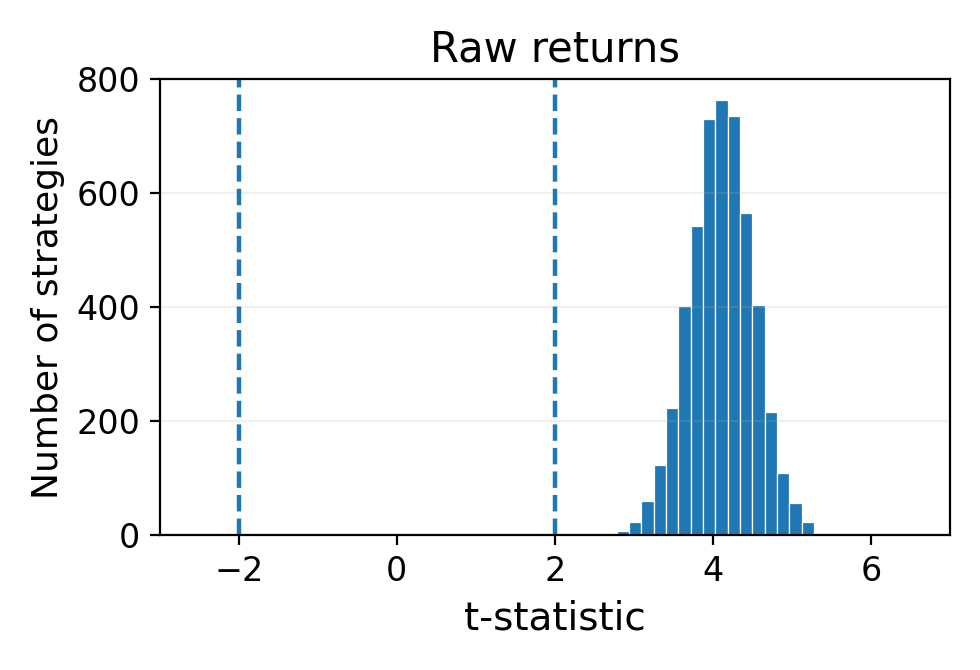
\includegraphics[width=.49\linewidth]{ps8_tstat_raw.png}\hfill
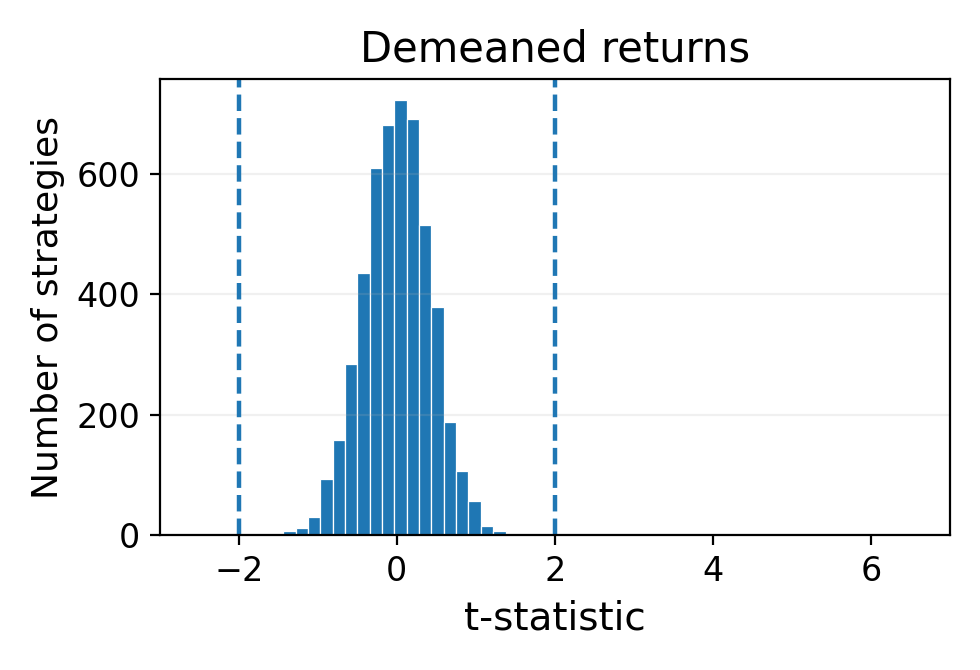
\includegraphics[width=.49\linewidth]{ps8_tstat_demeaned.png}
\caption{Full-sample $t$-statistics before and after portfolio-level demeaning.
Dashed reference lines are $-2$ and $+2$.}
\label{fig:g-hist}
\end{figure}

\paragraph{Comparison with the strategy from (e).}
We compared the random strategies with (e) over exactly the months that (e)
covers: the walk-forward training period (March 1953--June 2001, $T=580$) and
the held-out test period (July 2001--June 2026, $T=300$). In each window we drew
5,000 new random strategies with the same seed. The random strategies are not
charged trading costs, so comparing them only with the \emph{net} returns of (e)
would be unbalanced; Table~\ref{tab:gcompare} reports the gross comparison as
well. The CI limits are the 95\% intervals from (f), converted to monthly
Sharpe units.

\begin{table}[htbp]
\centering\small
\caption{Fraction of the 5,000 raw random strategies in each window whose Sharpe ratio exceeds that of the strategy in (e) or the upper end of its 95\% CI from (f). Random strategies have no trading-cost deductions.}
\label{tab:gcompare}
\begin{tabular}{llrrrr}
\toprule
Sample & (e) returns & Monthly SR & Annual SR & Beat (e) SR & Beat upper 95\% CI\\
 & & & & (\%) & Normal / General (\%)\\
\midrule
Training, 1953--2001 & Gross & 0.4429 & 1.5343 & 0.00 & 0.00 / 0.00\\
($T=580$) & Net & 0.3858 & 1.3365 & 0.00 & 0.00 / 0.00\\
\addlinespace
Test, 2001--2026 & Gross & 0.0996 & 0.3449 & 94.12 & 0.08 / 0.06\\
($T=300$) & Net & 0.0312 & 0.1081 & 100.00 & 39.94 / 40.04\\
\bottomrule
\end{tabular}
\end{table}

In the training window the average random strategy has a monthly Sharpe ratio
of 0.1370 (0.4746 annualized), and the highest is 0.203, below even the lowest
CI limit for (e), 0.290 (net, general). In the test window the average is
0.1379 (0.4778 annualized), and 81.94\% of random strategies have $|t|>2$
(84.12\% have $p<0.05$). The test CI upper limits are 0.2130 (normal) and
0.2133 (general) gross, and 0.14439 and 0.14436 net. Demeaning within the test
window makes only 10.8\% of random strategies beat the net SR of 0.0312, and
none beat the gross SR of 0.0996. This is a sensitivity check, \emph{not} a
risk-matched alternative, because it removes the premia from the random
portfolios but not from (e).

The comparison is not apples-to-apples. The random strategies are long-only
and benefit from the positive equity premia in the underlying portfolios.
The strategy in (e) is long seven portfolios and short seven with zero net
dollar exposure, which may reduce its market exposure but does not eliminate
systematic risk. The gap in Sharpe ratios therefore does not directly tell us whether the signals in (e)
are better or worse than random selection. The training-period comparison
is also biased in favor of (e): it combines several signals chosen from
full-sample results in (a), (b) and (d), and the rule was revised after earlier
test results had been viewed. The one-rule random strategies have no such
search behind them, so (e) beating all of them in training overstates its
merit. Its strong training and weak test performance illustrate selection
risk, not a clean, independently validated anomaly.

\paragraph{Bonus.}
The question does not fix the sample. We read ``the backtested Sharpe ratio''
as the one from the training period on which the rule was built, so our main
calculation uses the net walk-forward training returns (March 1953--June 2001,
$T=580$); the test period is reported briefly below. The largest monthly net
excess return is $+24.02\%$ (February 2000) and the smallest is $-17.06\%$
(March 2000). The mean is 1.243\% and the standard deviation 3.221\% per month,
so the monthly Sharpe ratio is 0.3858 (1.3365 annualized), and the two extremes
lie 7.07 and 5.68 standard deviations from the mean.

\emph{(a) Backtested Sharpe ratio taken as true.} We model monthly returns as
normal with standard deviation $\sigma$ equal to the sample value and mean
$\widehat{SR}\cdot\sigma$. A month at least as high as $+24.02\%$ then has
probability $7.7\times10^{-13}$, and a month at least as low as $-17.06\%$ has
probability $6.6\times10^{-9}$. Over 580 independent months, the chance of at
least one such month is $4.5\times10^{-10}$ and $3.9\times10^{-6}$.

\emph{(b) Any Sharpe ratio in the 95\% CI.} Holding $\sigma$ fixed and letting
the true Sharpe ratio range over the training interval from (f), the
upper-tail probability is between $4.2\times10^{-13}$ and $1.4\times10^{-12}$
for the normal interval (1.04 to 1.63 annualized) and between
$3.8\times10^{-13}$ and $1.5\times10^{-12}$ for the general interval (1.00 to
1.67). The lower-tail probability is between $4.0\times10^{-9}$ and
$1.1\times10^{-8}$ (normal) and between $3.8\times10^{-9}$ and
$1.2\times10^{-8}$ (general). A higher Sharpe ratio makes the maximum more
likely and the minimum less likely, but across the whole interval the
probabilities change only by a factor of about three to four. No plausible Sharpe ratio
makes the observed extremes likely under normality.

These extreme returns are difficult to reconcile with a normal model. The training
returns have kurtosis 11.1; six months lie more than four standard deviations
from the mean, against 0.04 expected under normality (seven lie beyond three,
against 1.6 expected). The two most extreme months occurred consecutively,
in February and March 2000, suggesting possible volatility clustering. The normal CI in (f) relies on the
same normality assumption, and both CIs assume independent months. A backtest
Sharpe ratio summarizes the mean and variance only: it says nothing about tail
risk, and the strategy with a 1.34 Sharpe ratio in training earned 0.11 in
the test period.

For the held-out test period ($T=300$), the extremes are $+16.90\%$ (March
2020) and $-14.79\%$ (April 2020), 4.38 and 3.89 standard deviations from the
mean. Under (a) their probabilities are $6.0\times10^{-6}$ and
$5.1\times10^{-5}$; over the (f) test intervals they range from
$3.6\times10^{-6}$ to $1.0\times10^{-5}$ and from $3.2\times10^{-5}$ to
$8.0\times10^{-5}$ (the normal and general intervals give the same values to
two significant digits). Four test months lie beyond three standard deviations,
against 0.81 expected.

\subsection*{AI Integration: Monte Carlo code check}

We expected the random strategies to show mostly positive and often
significant returns, since the underlying portfolios already had positive
average excess returns. After demeaning, we expected the $t$-statistics to move
closer to zero, with far fewer significant results.

We then asked an LLM to write the simulation. Its first script set seed 2026,
redrew a portfolio every month, and noted that the raw returns do not satisfy
a zero-mean null. But it omitted the workbook's second missing
code, $-99.99$, and reported 1,146 months. Its demeaned revision kept that
mistake. After we pointed out both missing codes, its third response used
1,124 complete months and found 100\% of raw versus 0\% of demeaned strategies
with $|t|>2$. We confirmed the corrected sample against the workbook. Our
simulation above uses our own code and a different seed (20261105), so we
report only our own statistics. Both simulations supported our prediction:
all raw strategies were significant, while none were after demeaning, an even
stronger result than we expected. As discussed above, positive premia explain
much of the raw significance. The initial error also shows why AI-generated
code still requires careful input validation. The three exchanges are summarized in
\texttt{ai\_process\_record.md}.

\subsection*{AI Integration: LLM strategy ideas and data snooping}

In response to the assigned short prompt, the LLM suggested ten strategies:
equal-weight, momentum, mean reversion, low-volatility, inverse-volatility,
minimum variance, risk-adjusted momentum, long--short momentum, time-series
momentum, and low-correlation diversification. Table~\ref{tab:g-ideas}
counts the main adjustable choices behind each idea. These are approximate
\emph{design choices}, not regression degrees of freedom or tests we ran.

\begin{table}[htbp]
\centering\scriptsize
\caption{Choices implicit in the ten LLM-proposed strategy families.}
\label{tab:g-ideas}
\begin{tabular}{p{.27\linewidth}p{.60\linewidth}r}
\toprule
Strategy & Examples of adjustable choices & Count\\
\midrule
Equal-weight & Universe, rebalancing frequency & 2\\
Momentum & Lookback/skip, top cutoff, weights, holding period & 4\\
Mean reversion & Lookback, bottom cutoff, weights, holding period & 4\\
Low-volatility & Volatility window, cutoff, weights, rebalancing & 4\\
Inverse-volatility & Volatility window, weight caps, floor, rebalancing & 4\\
Minimum variance & Covariance window, estimator, constraints, rebalancing & 4\\
Risk-adjusted momentum & Momentum/volatility windows, cutoff, weights & 4\\
Long--short momentum & Lookback, tails, exposure, weights, rebalancing & 5\\
Time-series momentum & Lookback, signal threshold, cash, weights & 4\\
Low-correlation diversification & Correlation window, selection, breadth, weights & 4\\
\bottomrule
\end{tabular}
\end{table}

The LLM \emph{did} warn about multiple testing, look-ahead bias, transaction
costs, and the need to test a chosen rule on untouched out-of-sample data. It
also recommended prioritizing four strategies, which could create another
selection stage. The full response and our evaluation are in
\texttt{ps8\_ai\_conceptual\_probe.md}. We did not record the model version,
and the reply mentions 75 portfolios although the prompt did not, so earlier
chat context may have shaped it.

Under an ideal zero-alpha null, ten fixed tests conducted at the 5\% level
would produce 0.5 false positives on average; if independent, the probability
of at least one is $1-0.95^{10}=40.1\%$. Tuning makes the count much larger.
If each choice in Table~\ref{tab:g-ideas} had just three settings, the ten
ideas would give about 900 variants and roughly 45 false positives at the
5\% level. These benchmarks assume a true null, so they do not describe our
raw Monte Carlo: there, any long-biased rule ``works'' because the portfolios
earn positive premia.

Trying many plausible rules and reporting only the winner is the file-drawer
problem: it overstates apparent Sharpe ratios and the published evidence for
anomalies. Before believing a result, we would want its full search history,
a stricter $t$-statistic hurdle (a Bonferroni-style cutoff rises from
$|t|\approx2.8$ for 10 tests to about 4.0 for 900), realistic risk and
implementation costs, and genuine out-of-sample validation.


\subsection*{References}
{\small Gultekin, M.\,N., and N.\,B.\ Gultekin (1983). Stock market seasonality: International
evidence. \textit{Journal of Financial Economics} 12(4), 469--481.\\[2pt]
Lo, A.\,W.\ (2002). The statistics of Sharpe ratios. \textit{Financial Analysts Journal}
58(4), 36--52.\\[2pt]
Mertens, E.\ (2002). Comments on variance of the IID estimator in Lo (2002). Working paper,
University of Basel.\\[2pt]
Opdyke, J.\,D.\ (2007). Comparing Sharpe ratios: So where are the p-values?
\textit{Journal of Asset Management} 8(5), 308--336.}

\end{document}
